\documentclass[10pt,a4paper]{article}
\usepackage[margin=14mm,top=12mm,bottom=12mm]{geometry}
\usepackage{fontspec}
\usepackage{xcolor}
\usepackage{graphicx}
\usepackage{hyperref}
\usepackage{array}
\usepackage{enumitem}

\setmainfont{Inter.ttf}[
  Path=assets/,
  BoldFont=Inter.ttf,
  BoldFeatures={FakeBold=1.2},
  ItalicFont=Inter.ttf,
  ItalicFeatures={FakeSlant=0.18},
  BoldItalicFont=Inter.ttf,
  BoldItalicFeatures={FakeBold=1.2,FakeSlant=0.18}
]
\setsansfont{Inter.ttf}[
  Path=assets/,
  BoldFont=Inter.ttf,
  BoldFeatures={FakeBold=1.2},
  ItalicFont=Inter.ttf,
  ItalicFeatures={FakeSlant=0.18},
  BoldItalicFont=Inter.ttf,
  BoldItalicFeatures={FakeBold=1.2,FakeSlant=0.18}
]
\setmonofont{DejaVuSansMono.ttf}[Path=assets/,Scale=0.82]

\definecolor{Purple}{HTML}{6047E8}
\definecolor{Lavender}{HTML}{CEC5FA}
\definecolor{Pale}{HTML}{F3F0FF}
\definecolor{Ink}{HTML}{18171D}
\definecolor{Muted}{HTML}{696776}
\definecolor{Line}{HTML}{E4E0F0}
\definecolor{CodeBG}{HTML}{F8F7FC}

\hypersetup{
  colorlinks=true,
  urlcolor=Purple,
  linkcolor=Purple,
  pdfauthor={OpenEd},
  pdftitle={Установка EdHarness и подключение OpenEd}
}
\pagestyle{empty}
\setlength{\parindent}{0pt}
\setlength{\parskip}{0pt}
\renewcommand{\familydefault}{\sfdefault}

\newcommand{\docheader}[1]{%
  \noindent\begin{minipage}[c]{0.72\linewidth}
    {\Large\bfseries\textcolor{Purple}{OpenEd}}\hspace{3mm}
    {\small\textcolor{Muted}{EDHARNESS · КРАТКОЕ РУКОВОДСТВО}}
  \end{minipage}\hfill
  \colorbox{Pale}{\strut\hspace{2mm}{\small\bfseries\textcolor{Purple}{#1}}\hspace{2mm}}\par
  \vspace{2mm}{\color{Lavender}\rule{\linewidth}{0.8pt}}\par\vspace{4mm}
}

\newcommand{\stephead}[2]{%
  {\fontsize{9}{10}\selectfont\bfseries\textcolor{Purple}{#1}}\hspace{2mm}%
  {\fontsize{14}{17}\selectfont\bfseries\textcolor{Ink}{#2}}\par\vspace{1.4mm}
}

\newcommand{\divider}{\par\vspace{3mm}{\color{Line}\rule{\linewidth}{0.65pt}}\par\vspace{3mm}}

\newcommand{\codebox}[2]{%
  \fcolorbox{Line}{CodeBG}{\parbox{\dimexpr#1-2\fboxsep-2\fboxrule\relax}{\vspace{1.5mm}\hspace{1.4mm}%
    {\ttfamily\fontsize{7.1}{9}\selectfont #2}\hspace{1.4mm}\vspace{1.5mm}}}%
}

\newcommand{\captionline}[1]{\vspace{1mm}{\fontsize{8}{10}\selectfont\color{Muted}#1}}

\begin{document}

\docheader{01 / 03}
{\fontsize{27}{31}\selectfont\bfseries\textcolor{Ink}{Установка и запуск}\par}
\vspace{1mm}{\small\color{Muted}Установите EdHarness и подключите аккаунт OpenEd.}\par
\vspace{3mm}

\noindent\begin{minipage}[t]{0.57\linewidth}
  \stephead{01}{Создайте аккаунт OpenEd}
  Откройте регистрацию и подтвердите адрес электронной почты.\par\vspace{3mm}
  {\large\bfseries\href{https://153.51.164.75/register}{Открыть регистрацию \ensuremath{\nearrow}}}\par
  \vspace{2mm}{\small\color{Muted}\url{https://153.51.164.75/register}}
\end{minipage}\hfill
\begin{minipage}[t]{0.37\linewidth}
  \vspace{1mm}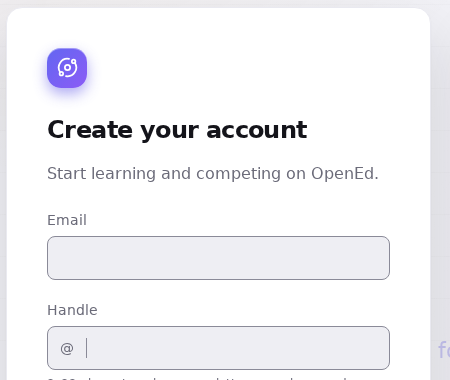
\includegraphics[width=\linewidth]{assets/register.png}
  \captionline{Страница регистрации OpenEd}
\end{minipage}

\divider

\stephead{02}{Установите Node.js и Git}
  Установите Node.js 24 LTS и Git. npm устанавливается вместе с Node.js.\par
  \vspace{1.5mm}{\small\href{https://nodejs.org/en/download}{Node.js}\quad\textcolor{Lavender}{/}\quad
  \href{https://git-scm.com/downloads}{Git}}\hfill
  {\ttfamily\small node -v\quad npm -v\quad git --version}

\divider

\stephead{03}{Установите EdHarness}
  Выполните команду в PowerShell, Terminal или другом терминале:\par\vspace{2mm}
  \codebox{0.99\linewidth}{\texttt{npm install -g --install-links --foreground-scripts "git+https://github.com/yarp-technologies/edharness.git\#edharness-v1"}}

\divider

\stephead{04}{Запустите EdHarness}
  Выполните команду в терминале:\par\vspace{2mm}
  \codebox{0.4\linewidth}{\texttt{\large edharness}}

\vfill
{\fontsize{8}{10}\selectfont\color{Muted}Для начала подключения используйте команду \texttt{/connect}.}

\newpage

\docheader{02 / 03}
{\fontsize{27}{31}\selectfont\bfseries\textcolor{Ink}{Подключение OpenEd}\par}
\vspace{1mm}{\small\color{Muted}Авторизуйте EdHarness и вернитесь в приложение.}\par
\vspace{3mm}

\stephead{05}{Откройте подключение}
  Введите \texttt{/connect} и выберите \textbf{OpenEd}. В окне авторизации нажмите \texttt{o} (open), чтобы открыть браузер.\par
  \vspace{2mm}
  \noindent\begin{minipage}[t]{0.485\linewidth}
    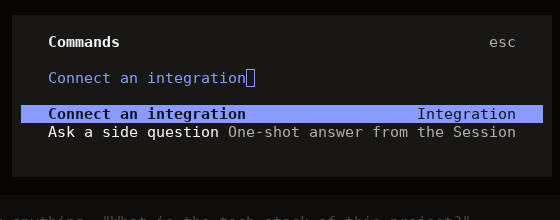
\includegraphics[width=\linewidth]{assets/connect-command.png}
    \captionline{Найдите Connect an integration}
  \end{minipage}\hfill
  \begin{minipage}[t]{0.485\linewidth}
    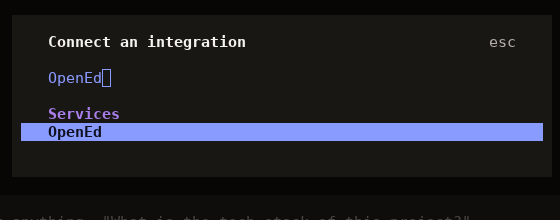
\includegraphics[width=\linewidth]{assets/opened-selected.png}
    \captionline{Выберите OpenEd}
  \end{minipage}
  \par\vspace{1.5mm}\noindent\hspace*{0.19\linewidth}%
  \begin{minipage}[t]{0.62\linewidth}
    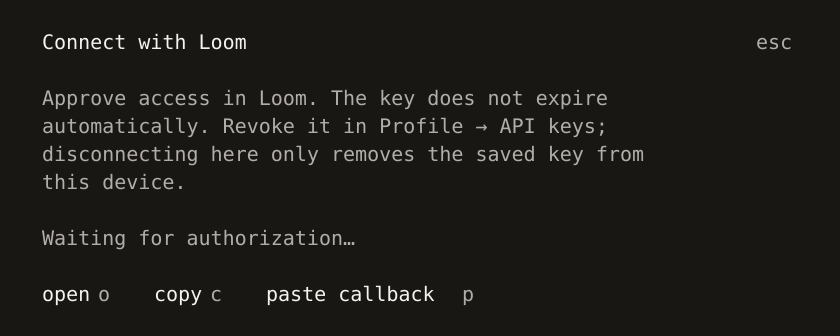
\includegraphics[width=\linewidth]{assets/opened-oauth-dialog.png}
    \captionline{Окно ожидания авторизации}
  \end{minipage}

\divider

\stephead{06}{Создайте ключ API}
  \noindent\begin{minipage}[t]{0.40\linewidth}
    \vspace{0pt}\raggedright
    Задайте имя ключа и максимальную роль.\par\vspace{2mm}
    Для всех доступных действий выберите \texttt{Select all permissions}; для ограниченного доступа отметьте нужные разделы. Оставьте обязательный доступ к LLM и нажмите \textbf{Create key and connect}.\par\vspace{2mm}
    \colorbox{Pale}{\parbox{0.96\linewidth}{\vspace{1mm}\small\textcolor{Purple}{Доступ к LLM обязателен для EdHarness.}\vspace{1mm}}}
  \end{minipage}\hfill
  \begin{minipage}[t]{0.56\linewidth}
    \vspace{0pt}
    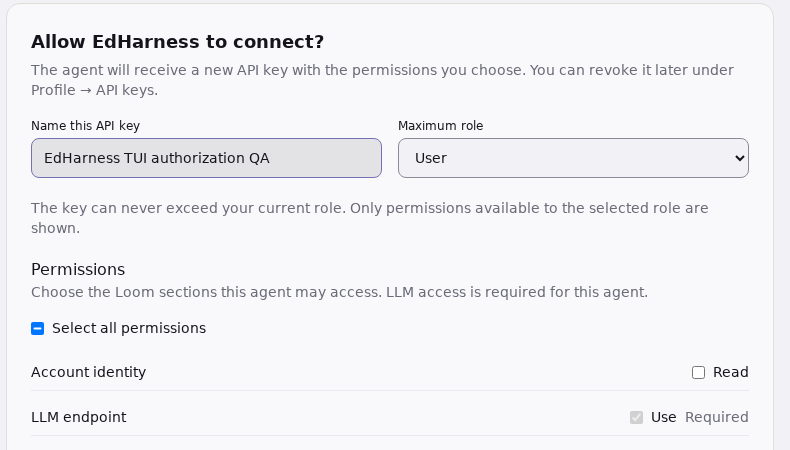
\includegraphics[width=\linewidth]{assets/permissions.png}
    \captionline{Выберите разрешения для ключа}
  \end{minipage}

\divider

\stephead{07}{Вернитесь в EdHarness}
  \noindent\begin{minipage}[t]{0.63\linewidth}
    \vspace{0pt}\raggedright
    Обычно браузер автоматически вернёт вас в EdHarness. Если перенаправления нет, скопируйте полный адрес из строки браузера. Он выглядит так:\par\vspace{1.5mm}
    \codebox{0.99\linewidth}{\scriptsize http://127.0.0.1:<порт>/oauth/callback?code=…\&state=…}\par\vspace{1.5mm}
    В TUI нажмите \texttt{p} → \textbf{Paste callback URL} и вставьте ссылку.\par\vspace{2mm}
    \small\color{Muted}Не публикуйте ссылку: в ней одноразовый код.
  \end{minipage}\hfill
  \begin{minipage}[t]{0.33\linewidth}
    \vspace{0pt}
    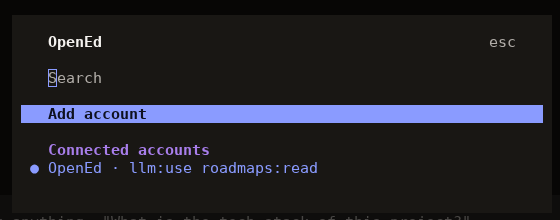
\includegraphics[width=\linewidth]{assets/connected-scope.png}
    \captionline{OpenEd подключён}
  \end{minipage}

\vfill
{\fontsize{8}{10}\selectfont\color{Muted}Готово: в списке подключений отображается OpenEd и доступный scope.}

\newpage

\docheader{03 / 03}
{\fontsize{26}{30}\selectfont\bfseries\textcolor{Ink}{Теперь можно пользоваться EdHarness}\par}
\vspace{1mm}{\small\color{Muted}Чтобы получить сведения из OpenEd, явно укажите OpenEd в запросе.}\par
\vspace{7mm}

\stephead{08}{Пример запроса к OpenEd}
  Напишите, что именно нужно найти в вашем аккаунте. EdHarness обратится к OpenEd и ответит по результату.\par
  \vspace{4mm}
  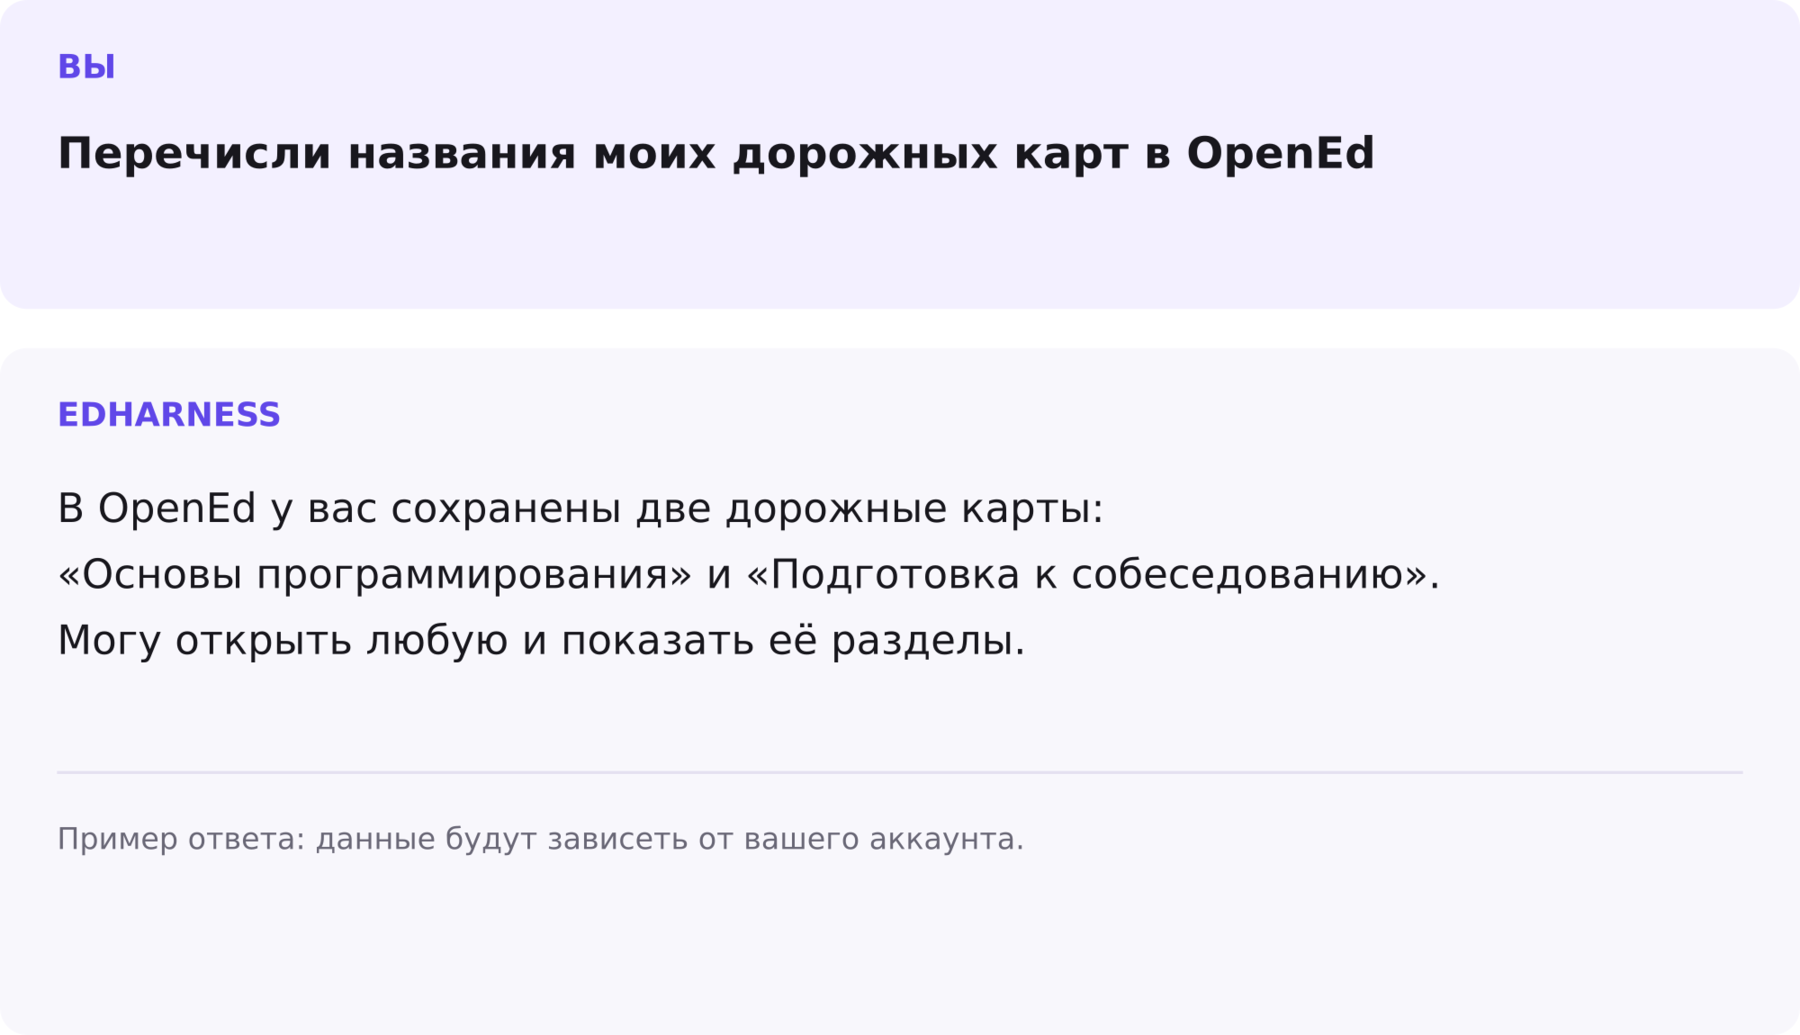
\includegraphics[width=0.98\linewidth]{assets/opened-api-example.png}\par
  \captionline{Пример ответа. Названия и количество дорожных карт зависят от вашего аккаунта.}

\vfill
{\fontsize{8}{10}\selectfont\color{Muted}Убедитесь, что при создании ключа были разрешены нужные разделы OpenEd.}

\end{document}
